\documentclass[11pt, a4paper]{article}

\usepackage{mlt-thesis-2015}

\usepackage[english]{babel}
\usepackage[hidelinks]{hyperref}
\usepackage{graphicx}
\usepackage{setspace}
\usepackage{comment}
\usepackage{caption}
\usepackage{listings}
\usepackage{textgreek}
\lstset{language=Python}

\usepackage[acronym]{glossaries}
\glsdisablehyper

\title{Implementing perceptual and spatial semantics in type theory with records (TTR)}
%\subtitle{An implementation of visual perception and spatial relations in \gls{ttr}}
\author{Arild Matsson}
\date{}

\newacronym{hmm}{HMM}{Hidden Markov Model}
\newacronym{lstm}{LSTM}{Long Short-Term Memory}
\newacronym{cnn}{CNN}{convolutional neural network}
\newacronym{ttr}{TTR}{type theory with records}
\newacronym{nlg}{NLG}{natural language generation}
\newacronym{vqa}{VQA}{visual question answering}
\newacronym{yolo}{YOLO}{You only look once}
\newacronym{nlp}{NLP}{natural language processing}

\begin{document}

%% ============================================================================
%% Title page
%% ============================================================================
\begin{titlepage}

\maketitle

\vfill

\begingroup
\renewcommand*{\arraystretch}{1.2}
\begin{tabular}{l@{\hskip 20mm}l}
\hline
Master's Thesis & 30 credits\\
Programme & Master’s Programme in Language Technology\\
Level & Advanced level \\
Semester and year & Spring, 2018\\
Supervisors & Simon Dobnik and Staffan Larsson\\
Examiner & (name of the examiner)\\
Keywords & type theory, image recognition, object recognition, perceptual semantics, visual question answering
\end{tabular}
\endgroup

\thispagestyle{empty}
\end{titlepage}

%% ============================================================================
%% Abstract
%% ============================================================================
\newpage
\singlespacing
\glsresetall
\section*{Abstract}

\Gls{ttr} combines several theories of semantic modeling in a single framework.
[more ttr appraisal: type checking, robustness, verifiable...]
The present work suggests a \gls{ttr} model of perception, spatial cognition and language.
Utilizing PyTTR, a Python implementation of \gls{ttr}, the model is then implemented as an executable script.
%The Python implementation includes reformatting the output of an external image recognition system and parsing natural language.
Over pure Python programming, \gls{ttr} provides a transparent formal specification, as well as advanced typing and type checking.
The implementation is evaluated in a \acrlong{vqa} task.
The results confirm the suitability of this approach.
... as well as identifying some desired additions to PyTTR.
... machine learning??

% TTR also provides a connection between perception and a wide range of semantic phenomena described in TTR, e.g. quantification, inference, modality, negation, semantic coordination,.

\thispagestyle{empty}

%% ============================================================================
%% Preface
%% ============================================================================
%\newpage
%\section*{Preface}

%Acknowledgements, etc.

%\thispagestyle{empty}

%% ============================================================================
%% Contents
%% ============================================================================
\newpage

\begin{spacing}{0.0}
\glsresetall
\tableofcontents
\end{spacing}

\thispagestyle{empty}

%% ============================================================================
%% Introduction
%% ============================================================================
\newpage
\setcounter{page}{1}

\glsresetall
\section{Introduction}
\label{sec:intro}

Having computers "understand" images is desirable in several areas.
In this context, understanding means to process visual input on a cognitive level.
Sub-cognitive image processing may include tasks such as prominent color extraction, edge detection and visual pattern recognition.
Cognitive processing, however, includes identifying objects, their properties and their relations to each other, as well as including this information in further cognitive processes, such as reasoning and prediction [sources?].
This is a requirement for some (camera-equipped) robots in order to obtain knowledge (or beliefs) and select appropriate actions: domestic assistants [src?], driver-less cars [src?] to name a few examples.
The same kind of processing can also be used outside situated agents, for automatic processing of large sets of visual data [?].

[the creation of ttr]

The theoretical background for this thesis is summarized in \textit{Background}.
In the \textit{Method} section, a model is defined and its implementation in Python and PyTTR described.
Then follows an account of the \textit{Results} with discussion, and finally some \textit{Conclusions}.
[enable numbered sections instead]

\glsresetall
\section{Background}
\label{sec:background}

This section will highlight some important pieces of the history of past research in relevant fields.

\subsection{Computational semantics}

Philosophers have long been interested in the study of meaning.
[Frege, ...]

Computational accounts of meaning emerged [how].
They are/were characterized by [what].
[Montague, ...]
[FOL]

With recent advancements in computer science, ambitious computational-semantic theories are now in abundance.
As a competitor to formal systems, statistical methods have emerged which do well in various tasks within semantics, leveraging the large amounts of digital data that are available as a product of our largely digitalized society.

If statistical models of semantics do well in [empirical/data-driven/practical] tasks, formal theories of semantics [do what?]
\cite{BlackburnComputationalsemantics2003}:
FOPC for the win, but "other approaches are both possible and interesting".



\subsubsection{Perceptual semantics}

\cite{HarnadSymbolGroundingProblem1990}

\cite{LoganComputationalAnalysisApprehension1996}:
Basic–deictic(–intrinsic) relations.
Perceptual–conceptual representation.
"Computational theory of apprehension": spatial indexing -> reference frame -> ... Instead, we move into the conceptual level, both in perception and language, and evaluate validity from there.
(Drawbacks?)
They present "evidence" for their theory, does that evidence contradict the present approach?

\cite{RegierGroundingspatiallanguage2001a}:
Four models. AVS.
Many experiments.
Spatial term ratings influenced by: proximal \& center-of-mass orientations, grazing line, distance.

[functional aspect, Coventry?]

[mention grounding!?]

[vqa]



\subsubsection{Computer vision and object recognition}

[computer vision]

You only look once (YOLO) \citep{RedmonYouOnlyLook2015} is a neural network model that simultaneously predicts bounding boxes around objects and classifies the contained objects.

Among the most recent contributions to computer vision, Facebook's \textit{Detectron} \citep{Detectron2018} features outlining of identified objects and classification with impressive accuracy.

\begin{figure}[h]
\label{fig:dogbike_annotated}
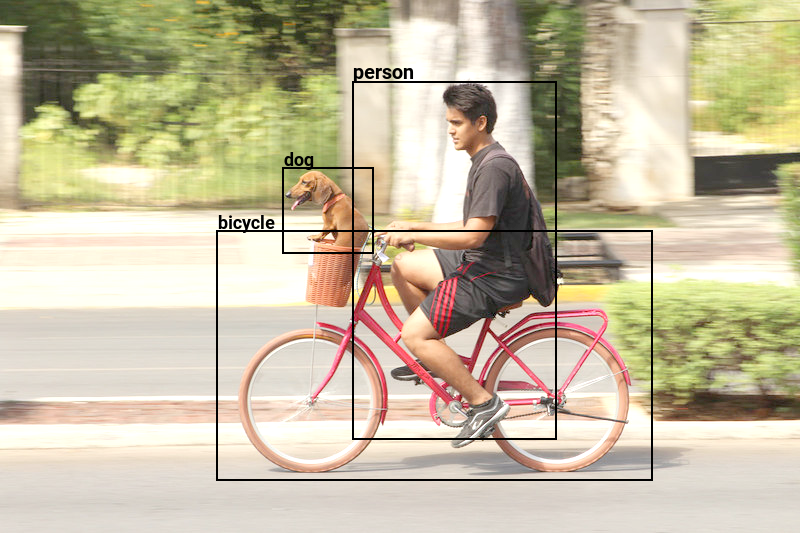
\includegraphics[width=\textwidth]{dogbike_annotated}
\centering
\caption{Visualization of the labels and bounding boxes emitted by YOLO when given an image depicting a cyclist with a dog.}
\end{figure}



\subsection{Type theory in natural language processing}

Type theory was developed as an alternative to set theory, responding to paradoxes found in the latter.
With set theory widely serving as a \textit{foundation of mathematics}, the development of this new theory was [important].
Several different type theories have been created, of which Church's \textit{simply typed \textlambda-calculus} \cite{church40} and Martin-Löf's \textit{intuitionistic type theory} \citep{martinlof84} are some prominent examples.
\citep{CoquandTypeTheory2015} [too detailed?]

[use of type theory in nlp]

\cite{CooperRecordsRecordTypes2005} combines several theories from logic, semantics and linguistics in a single framework called \textbf{\acrfull{ttr}}.
 lambda calculus, phrase structure grammar, (DRT), (situation semantics) (what are the latter)?
It has been employed to model natural language in the context of dialogue, situated agents and spoken language.

[brief summary of TTR syntax?]



\subsubsection{Applications of \gls{ttr}}

\cite{LarssonDialoguesHaveContent2011}

\cite{DobnikModellinglanguageaction2012}

\cite{lspc} model the point space perception of a mobile robot equipped with a rangefinder.
 that would move around and use laser range scanner or similar to collect points in space, group them into objects and detect spatial relations between them.
\Gls{ttr} is mainly used to model the transition from the perceptual to the cognitive domain as well as 
 throughout the model, accounting for perception and cognition.

\cite{ttrspat} develop this further, focusing especially on spatial relations.

\cite{LarssonFormalsemanticsperceptual2015}

Parsing: \cite{CooperRecordsRecordTypes2005}, \cite{RobinCooperAustiniantruthattitudes2005}, \cite{CooperTypetheorysemantics2012}, \cite{CooperTypetheorylanguage2016}



\subsubsection{PyTTR}

\cite{pyttr} is a Python implementation of \gls{ttr}.
It supports modeling records, record types, ptypes, functions and other TTR objects.
Additionally, it allows operations such as judgement, type checking and subtype checking.
As a Python library it also enables other features and peripheral procedures to be written in Python.

[the advantage of implementing a theoretical model]
PyTTR, itself being an implementation of TTR, allows, in turn, the implementation of models and theories that build on TTR.
By implementing a theoretical model as a computer program, it can "come alive" and be tested on real problems and data.
Another motivation for implementation is to compete with existing, less theoretically strong techniques to solve a given task, but it is possibly secondary to the former reason.

%[What has been written in PyTTR so far? nu, animat]



\section{Method}
\label{sec:method}

"we are using TTR as a formal specification language that tell us how to do visual question answering in Python. This additional layer gives us a formal transparency and the ability to type check the code before running it." (SD)

Goal: Implement \cite{ttrspat}.
Except we 1) do images and 2) add language.
We do images because a) it's interesting to look at another medium and b) it's easier to get data? c) to do vqa.
We add language because we're just really interested in language.
We don't take it very far in that direction, though, just the basics.

%To connect more with the linguistics of spatial semantics, we added simple parsing and validation of natural-language propositions/questions.

%Below, we first develop on the theory of object recognition and spatial descriptions, in terms very similar to \cite{ttrspat}, but with our own additions and modifications as appropriate.
%Then we describe how implementation was done, focusing especially on some details that were not straightforward.



\subsection{Theory development}
\label{ssec:theory}

The different input space implies a different type of location data.
Spatial relation classification is simplistic.
In the end, language input is added.
[...]

To collect the various parts as a united whole, we create an agent.
[...]



\subsubsection{Concepts of objects}
% Distinguish different uses of "object": TTR a:T, Obj, IndObj.

The term \textit{object} occurs in various fields with different meanings, and it is overloaded within this thesis as well.
In \gls{ttr}, an object is something that belongs to the extension of a type.
In computer vision, an object can be detected in a certain location within an image, and subsequently classified.
[...]



\subsubsection{Spatial relations}
% Classification algorithm non-TTR. Simplistic, compare to sophisitcated alternatives.



\subsubsection{Language}
% Why connect language? Is it VQA? Parsing. Classification before or after question.



\subsubsection{Implementation plan}
% How did I go about to implement this? PyTTR, YOLO, 




The $Obj$ type couples a property with a location, but it does not explicitly say anything about any individual object.
In \cite{lspc}, this corresponds to a \textit{perceptual} notion.
The step to the \textit{conceptual} domain is marked by generating a record type that corresponds to a situation, namely the situation that a certain individual has a certain property and is at a certain location.
%This is the \textit{basic relation} in \cite{LoganComputationalAnalysisApprehension1996}.
Such a situation type is defined in \autoref{eq:indobj} as $IndObj$.
It follows a typical pattern in \gls{ttr} litterature, with a set of fields declaring basic objects and another set of fields defining constraints, or predicates, on the basic objects.
In this case, $x$ is an individual and $loc$ is a location.
$cl$ specifies that $loc$ is the location of $x$, and the purpose of $cp$ is to declare a property of $x$.
(Had TTR allowed it, we could have been more specific by stating that the field $cp$ should be of a ptype dependent on the field $x$.)

\begin{equation}\label{eq:indobj}
IndObj = \left[\begin{array}{rcl}
\text{x} &:& Ind \\
\text{loc} &:& Segment \\
\text{cp} &:& Type \\
\text{cl} &:& \text{location}(\text{x}, \text{loc}) \\
\end{array}\right]
\end{equation}

The function for generating an $IndObj$ subtype from an $Obj$ record is known from \cite{lspc} as an \textit{individuation function}.
It will be of the type $IndFun$.

\begin{equation}\label{eq:indfun}
IndFun = ( Obj \rightarrow RecType )
\end{equation}

As a constraint that cannot be expressed in TTR, the record type resulting from applying an $IndFun$ function should be a subtype of $IndObj$.
[How about a notation $RecType_{\sqsubseteq IndObj}$ "the type of all record types which are subtypes of $IndObj$"?]



\subsubsection{Proof objects and singleton record types}

The type of the individuation function was given above.
But before a definition of it can be given, we need to dive deeper into some \gls{ttr} concepts.

There is a certain notable difference between the types $Obj$ and $IndObj$.
The former is a single record type, of which there will be many records.
Each record will hold information about a given detected object.
With the latter, it is the type itself that holds meaning, by describing a situation.
However, note that the $cp$ field is only being declared generally as $Type$.
Thus, it is \textit{subtypes} of $IndObj$, with a more specific typing of $cp$, that will be truly informative.

[propositions as types, true if there is an object of the type, situation semantics? \cite{BarwiseSituationsAttitudes1981}]
A record of a situation type then serves as a witness for the situation.

For each record type returned by the individuation function, a record is simultaneously created.
The $loc$ value of this record is naturally identical to the $seg$ value of the $Obj$ input record.
Objects for the remaining fields need to be instantiated on the spot.
Object creation is notated here as $A_{new}$, where the symbol $A$ may vary for the sake of readability.
%For the $x$ field, we create a new individual object $a_{new} : Ind$.
%For the ptype fields $cp$ and $cl$, we also create new objects $e_{new} : r.\text{pfun}(\text{x})$ and $e_{new} : \text{location}(\text{x}, \text{loc})$.

We are now ready to define the individuation function as in \autoref{eq:indfundef}, with an example application in \autoref{eq:indfunrec}.
The definition uses manifest fields to denote the \textit{fully specified} record type, or singleton record type.

\begin{equation}\label{eq:indfundef}
\lambda r : Obj\ . \left[\begin{array}{lcl}
    \text{x} = a_{new} &:& Ind \\
    \text{cp} = e_{new} &:& r.\text{pfun}(\text{x}) \\
    \text{cl} = e_{new} &:& \text{location}(\text{x}, \text{loc}) \\
    \text{loc} = r.\text{seg} &:& Segment\\
\end{array}\right]
\end{equation}

\begin{equation}\label{eq:indfunrec}
\left[\begin{array}{rcl}
\text{seg} &=& \left[\begin{array}{rcl}
\text{cx} &=& 138\\
\text{w} &=& 276\\
\text{cy} &=& 654\\
\text{h} &=& 809
\end{array}\right]\\
\text{pfun} &=& \lambda v:Ind\ .\ \text{person}(v)\\
\end{array}\right]
\mapsto
\left[\begin{array}{lcl}
    \text{x} = a_0 &:& Ind \\
    \text{cp} = e_0 &:& \text{person}(\text{x}) \\
    \text{cl} = e_1 &:& \text{location}(\text{x}, \text{loc}) \\
    \text{loc} = \left[\begin{array}{rcl}
\text{cx} &=& 138\\
\text{w} &=& 276\\
\text{cy} &=& 654\\
\text{h} &=& 809
\end{array}\right] &:& Segment\\
\end{array}\right]
\end{equation}

\begin{comment}
From a fully specified record type, the one record that it describes can be \textit{instantiated}.
[define formally?]
[wait, it's already called \textit{extension}]

\begin{equation}
\left[\begin{array}{rcl}
\text{x} = a &:& Ind\\
\end{array}\right]
\mapsto
\left[\begin{array}{rcl}
\text{x} &=& a\\
\end{array}\right]
\end{equation}

The \textbf{generalization} of a record type $T$ is a record type whose fields are the same as $T$ except that singleton fields are replaced by non-singleton fields. In other words, it is $T$ with manifest fields removed.

\begin{equation}
\left[\begin{array}{rcl}
\text{x} = a &:& Ind\\
\end{array}\right]
\mapsto
\left[\begin{array}{rcl}
\text{x} &:& Ind\\
\end{array}\right]
\end{equation}
\end{comment}



\subsubsection{Spatial relations}

Between any pair of individuals, a relation may hold.
Our concept of individuals is now a collection of fully specified $IndObj$ record types.
How do we detect and model a certain relation between such a pair?

Since we are interested in the spatial relation between a \textit{reference object} and a \textit{located object}, we will be constructing tuple-like records of the type $LocTup$ defined in \autoref{eq:loctup}.
Records of this type contain instantiations of two $IndObj$ record types.
In \autoref{eq:clf}, a classifier is modeled as a function from such a record to a new record type which should describe the relation.

\begin{equation}\label{eq:loctup}
LocTup = \left[\begin{array}{rcl}
    \text{lo} &:& IndObj \\
    \text{refo} &:& IndObj \\
    \end{array}\right]
\end{equation}

\begin{equation}\label{eq:clf}
ClfFun = ( LocTup \rightarrow RecType )
\end{equation}

For instance, a classifier for "to the left of" might look like in \autoref{eq:leftclfdef}, where $\kappa_{left}$ is a non-TTR, boolean function.
Of course, the requirement that the individual $r.\text{lo}.\text{x}$ is actually located at $r.\text{lo}.\text{loc}$ (and same for $r.\text{refo}$) is implicit from the typing as $IndObj$, where the field $\text{cl} : \text{location}(\text{x}, \text{loc})$ is necessarily present.

\begin{equation}\label{eq:leftclfdef}
\lambda r : LocTup \ .\ 
\begin{cases}
\left[\begin{array}{rcl}
    \text{cr} &:& \text{left}(r.\text{lo}.\text{x}, r.\text{refo}.\text{x}) \\
\end{array}\right],
& \text{if } \kappa_{left}(r.\text{lo}.\text{loc}, r.\text{refo}.\text{loc}) \\
[], & \text{otherwise}
\end{cases}
\end{equation}

[move this paragraph to Discussion?]
\cite{ttrspat} includes two important aspects that are not covered here.
First, it assumes a 3D point space as visual input, in contrast to the 2D image considered here.
Spatial relations in 3D crucially involves adapting the reference frame according to the viewpoint, while those are trivially fixed in the 2D case.
Second, it accounts for the functional aspect of spatial relationship, as detailed by \cite{CoventryClassificationExtrageometricInfluences2004}.



\subsubsection{Language}

[highlight how TTR makes it easy to answer a yes/no question]

A dog is to the left of a car
\begin{equation}\left[\begin{array}{rcl}
\text{x} &:& Ind\\
\text{y} &:& Ind\\
\text{c}_\text{dog} &:& \text{dog}(x)\\
\text{c}_\text{car} &:& \text{car}(y)\\
\text{c}_\text{left} &:& \text{left}(x, y)\\
\end{array}\right]\end{equation}


Essentially, we would like to check if the situation observed is a subtype of the situation described by the text/question, whether $Q \sqsupseteq A$. A new problem here is that field labels do not match, even if the field values (the types) match. We thus need to consider all (?) relabelings of $Q$:

A record type $T_1$ is a \textbf{relabel-subtype} of $T_2$, or $T_1 \sqsubseteq_{rlb} T_2$,  iff there is a relabeling of $T_1$, $T_{1_{rlb}}$ where $T_{1_{rlb}} \sqsubseteq T_2$.

(Or: iff $T_1$ is $\Sigma$-equivalent to a subtype of $T_2$?)

Could we forget field labels and just look at the two sets of field values? Not really, because we have dependent types, so $\text{dog}(x_1) ≠ \text{dog}(x_2)$. We need to carry out each candidate \textit{relabeling} and check subtypeness. In practice, and in this case, relabeling the basic-type ($Ind$) fields is enough, because those are the only ones whose labels appear in dependent fields. For each basic-field relabeling, we can then kind of forget labels and just find subtypeness of field values.

[Relabel-subtype pseudocode]



\subsubsection{Agent}

The perceptual-conceptual pieces described above are here combined.
We are building an agent who receives classified and located objects of an image, apprehends their basic status and spatial relations, and validates natural-language propositions.

\begin{equation}\label{eq:agent}
Agent = \left[\begin{array}{rcl}
    \text{objdetector} &:& ObjDetector \\
    \text{indfun} &:& IndFun \\
    \text{appr} &:& [(Rec \rightarrow RecType)] \\
    \text{state} &:& AgentState \\
    \end{array}\right]
\end{equation}

\begin{equation}\label{eq:state}
AgentState = \left[\begin{array}{rcl}
    \text{img} &:& Image \\
    \text{perc} &:& [Obj] \\
    \text{bel} &:& [RecType] \\
    \text{utt} &:& RecType \\
    \end{array}\right]
\end{equation}

The fields $objdetector$, $indfun$ and $appr$ of $Agent$ are to be statically defined for a specific agent.
While running, the agent will modify the $AgentState$ record in $state$.

\begin{enumerate}
\item Visual input in the form of an image is received and assigned to $state.img$.
\item $objdetector$ is invoked on $state.img$ and creates a collection of records that are assigned to $state.perc$.
\item $indfun$ is, in turn, invoked on each record in $state.perc$ and resulting record types are added to $state.bel$.
\item Now, the functions in $appr$ are applied to type-valid combinations of $state.bel$ records, and resulting record types are added to $state.bel$
	\begin{enumerate}
	\item Define "type-valid combinations"? How detailed?
	\end{enumerate}
\item Any language input is parsed and the resulting record type assigned to $state.utt$.
\item The record types in $state.bel$ are combined/concatenated. If the resulting record type is a relabel-subtype of $state.utt$, a positive answer is emitted; otherwise a negative answer is emitted.
\end{enumerate}



\subsection{Implementation}

Much of the theory developed above is straightforwardly implemented in PyTTR.
Python is used mostly for binding the pieces together, but also some significant processes.



\subsubsection{Invoking YOLO}

YOLO \citep{yolo} is made with C but there is a Python wrapper.
When invoked from Python, the return value is a collection of dict objects with field for label, coordinates and a confidence score.
I made a Python function which takes this collection and translates it to a list of PyTTR $Obj$ records.

\begin{comment}
\begin{lstlisting}[language=Python]
from darkflow.net.build import TFNet
import numpy as np

tfnet = TFNet({"model": "yolo/yolo.cfg", "load": "yolo/yolo.weights",
    'config': 'yolo', "threshold": 0.2})

yolo_out = dict()
def yolo(img):
    """Invokes YOLO on a PIL image, caches and returns the result."""
    if str(img) not in yolo_out:
        yolo_out[str(img)] = tfnet.return_predict(np.array(img))
    return yolo_out[str(img)]

def yolo_coords(o):
    """Extract YOLO output coordinates as ((x0,y0), (x1,y1))."""
    return (o['topleft']['x'], o['topleft']['y']),
        (o['bottomright']['x'], o['bottomright']['y'])

def xy1xy2_to_cwh(x1, y1, x2, y2):
    '''Transform to center, width and height.'''
    return {'cx': int(x1/2 + x2/2), 'cy': int(y1/2 + y2/2),
        'w': x2 - x1, 'h': y2 - y1}

def yolo_detector(i):
    """Creates IndObj records for YOLO results."""
    return [Rec({
        'seg': Rec(xy1xy2_to_cwh(
            *yolo_coords(o)[0], *yolo_coords(o)[1])),
        'pfun': create_fun(o['label'].replace(' ', '_')),
    }) for o in yolo(i)] # @todo RBG/BGR?
ObjDetector.witness_cache.append(yolo_detector)
\end{lstlisting}
\end{comment}



\subsubsection{Spatial classifiers}

Spatial classifiers $\kappa$ are typed as $(Segment \rightarrow Segment \rightarrow bool)$.
I have implemented them as Python functions.
For the purpose of this thesis, no sophisticated spatial classification has been considered.
Instead, a naive comparison between centers of bounding boxes was implemented.
This was done for the four relations "left", "right", "above" and "below".



\subsubsection{Natural language parsing}

Parsing text to TTR has been addressed in \cite{CooperRecordsRecordTypes2005}, \cite{RobinCooperAustiniantruthattitudes2005}, \cite{CooperTypetheorysemantics2012}, \cite{CooperTypetheorylanguage2016}.
These accounts cover basic grammar, and are likely enough for the kind of utterances considered here.
It would have been interesting to see also those implemented here.
However, to save time I went for a simpler approach using NLTK's feature structure CFG.
With a custom Python function, the FOPC output is transformed to a TTR record type.



\subsubsection{Where PyTTR is not enough}

The individuation function, although expressible in TTR, is not possible to implement in PyTTR.
Therefore, it was implemented as a Python function named {\tt individualize}.

The \textit{relabel-subtype} relation, $\sqsubseteq_{rlb}$, was also implemented in Python.



\subsection{Evaluation}

[test on a few images and sentences] [or is one enough? it does what it does...]



\section{Results}
\label{sec:results}




\subsubsection{Objects}

We begin the model formulation by declaring three basic types.

\begin{description}
\item [$Int$] An integer, such as 415.
\item [$Image$] A 2-dimensional digital image. It serves as an identifier to a set of extracted information, and its file type and actual data is not important in this thesis.
\item [$Ind$] A single individual object (or person), such as the reader or the Eiffel Tower.
\end{description}

A $Segment$ is a record type describing a rectangular bounding box within an (implicit) image (\autoref{eq:seg}).
$Ppty$ is the type of functions that can be applied to an individual and return a type (\autoref{eq:ppty}).
In our account the resulting type will be restricted to a ptype that is dependent on the individual, thus describing a property of it.

\begin{equation}\label{eq:seg}
Segment = \left[\begin{array}{rcl}
\text{cy} &:& Int\\
\text{cx} &:& Int\\
\text{w} &:& Int\\
\text{h} &:& Int
\end{array}\right]\end{equation}

\begin{equation}\label{eq:ppty}
Ppty = (Ind \rightarrow Type)\end{equation}

An object that has been detected in an image is, at the perceptual level, modeled as a record of the type $Obj$, essentially a tuple of a position and a semantic property (\autoref{eq:obj}).
An example $Obj$ record is given in \autoref{eq:objrec}.
$Obj$ records are the result of performing \textit{object detection}.
This fact is expressed in TTR as the function type $ObjDetector$ (\autoref{eq:objdetector}).

\begin{equation}\label{eq:obj}
Obj = \left[\begin{array}{rcl}
\text{seg} &:& Segment\\
\text{pfun} &:& Ppty \\
\end{array}\right]\end{equation}

\begin{equation}\label{eq:objrec}
obj =
\left[\begin{array}{rcl}
\text{seg} &=& \left[\begin{array}{rcl}
\text{cx} &=& 138\\
\text{w} &=& 276\\
\text{cy} &=& 654\\
\text{h} &=& 809
\end{array}\right]\\
\text{pfun} &=& \lambda v:Ind\ .\ \text{person}(v)\\
\end{array}\right] : Obj\end{equation}


\begin{equation}\label{eq:objdetector}
ObjDetector = ( Image \rightarrow [Obj] )
\end{equation}




\subsection{Discussion}
\label{sec:discussion}

Contradiction of Logan \& Sadler's "evidence" for their "theory of apprehension" (which is different from mine)?

...



\section{Conclusions}
\label{sec:conclusions}

It works and it's nice because...



\subsection{Future work}

Spatial templates \& regions of acceptability. Compound relations (above right) finer (directly). Functional aspect.  \cite{LoganComputationalAnalysisApprehension1996} (also Dobnik etc)

Basic->Deictic->Intrinsic relations  \cite{LoganComputationalAnalysisApprehension1996}. 3D.

4 question types.
Moar question types (tasks/programs/routines in L\&S).

Dialogue.

Classification after Q.

Probabilistic TTR for "good fit" (is is more to the left or more above?).



\bibliography{imagettr}
\end{document}